\documentclass[10pt,twocolumn,a4j]{jarticle}
\usepackage[dvipdfmx]{graphicx}
\huge
\title{\normalsize \textbf {DAOにおける内部告発の提案}}
\author{\normalsize	情報・通信工学科 荒木研究室所属 182C1117 津田匠貴}
\date{}
\begin{document}
\maketitle
\section{\normalsize はじめに}
DAO(Decentralized Autonomous Organization:自立分散型組織)は経済的な共通目的を持った匿名個人らが中央集権的な管理主体を持たず
に活動を行う組織であり,独自トークンの発行や分散台帳としての記録機能をもつブロックチェーン技術の使用を前提に成り立っている.

多くのDAOでは自立分散的に機能するまで株式会社などの中央集権的組織が主体となって運営しているが,彼らによる資金の持ち逃げといった問題が数多く発生している.
不正を防止し,コミュニティによる分散的統治を実現するために,本研究ではEthereumブロックチェーンにおいて秘密分散法を用いたメンバーシップの導入と内部告発機能を提案する.
これは不正を行う兆候があるユーザーを検知した場合に内部告発を行い,メンバーの投票による審議を行うことで,不正を防止するスキームを目指している.

\section{\normalsize シャミアの秘密分散法}
シャミアの秘密分散法では,ある秘密を分散情報として管理し,事前に定めた閾値以上の分散情報が集まった場合にのみ復元できるという仕組みである.
各メンバーを$U_1,...,U_n$とし,素数$p(n<p)$,秘密$s(s∈Z_p)$としたとき,各$U_i$には$d_i∈Z_p$が割り当てられる.
また,秘密を分散し,配布する役割を担うディーラー$D\notin{{U_1,...,U_n}}$としたとき,
シャミアの秘密分散法における流れは以下のようになる.
\begin{enumerate}
  \item $D$は各$1≦j≦t-1$について,秘密かつ無作為に$a_j∈Z_p$を選び,式(1)のような多項式を定める.
        \begin{equation}
          f(x)=s+a_1x+a_2x^2+...+a_{t-1}x^{t-1}
        \end{equation}

        このとき,秘密$s$について,$s=f(0)$である.
  \item $D$は$U_i$に$s_i=f(d_i)$を送る.
  \item 任意の$t$人のメンバー$U_{i1},...,U_{it}$は式(2)のラグランジュ補間公式を用いることで秘密を復号することができる.
        \begin{equation}
          s=\sum^t_{{k=1}}s_{i_k}\prod_{1≦\ell≦t,\ell≠k}\frac{d_{i_\ell}}{d_{i_\ell}-d_{i_k}}\rm{mod}\;p
        \end{equation}

\end{enumerate}

\section{\normalsize メンバーシップの提案}
DAOにおいて内部告発を実現する場合,以下の二つの条件が矛盾する.
\begin{enumerate}
  \item 全てのメンバーが匿名環境下で活動できる
  \item 不正を行う疑いがあるメンバーを特定する
\end{enumerate}
また,内部告発の対象となる資金の持ち逃げは,資金を取り戻すことはほぼ不可能であるため,
インシデントが起きる前に不正を防ぐ必要がある.

そのような不正をWeb3上から事前に察知するのは困難だが,Web2上のコミュニケーションツールのチャット内容などから推測できるので,
予めWeb2上のアカウントとWeb3上のアカウントを紐付け,Web2上のアカウントが公開された場合にのみWeb3上のアカウントを特定でき,罰則を与える構図を考えた.

このようなスキームであれば,不正を行うリスクが生まれるため,そのような行いを起こそうとするメンバーに対するディセンティブ機構として機能することが期待できる.
また,上述の矛盾を緩和することができる.
\begin{figure}[htbp]
  \begin{center}
    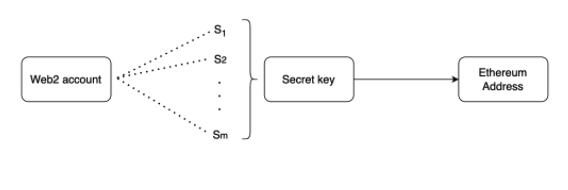
\includegraphics[width=80mm]{account.png}
    \caption{アカウント管理モデル}
  \end{center}
\end{figure}
このモデルはシャミアの秘密分散法を用いており,全てのメンバーは以下の流れに従いアカウントを登録する.
\begin{enumerate}
  \item Ethereum Addressを作成する際に使った秘密鍵を$m$個のsecret shareに分割する
  \item 1つのWeb2 accountにつき,$m$個のsecret shareを紐付けたペアを作る
  \item それぞれのペアは$m$人のメンバーに配られる
\end{enumerate}
これにより,閾値$n$個以上のペアが集まればラグランジュ補間公式より,自身の秘密鍵が復元されEthereum Address上の資産を失うなどのリスクを追うことになる.
このようなリスクを回避する唯一の方法は,自身が内部告発の対象にならないことであり,Web2上で誠実な振る舞いを続け,DAOにとって危害を与えるような言動を慎むことである.

\section{\normalsize まとめ・今後の展望}
本研究では,DAOにおけるコアメンバーへの牽制を意図した内部告発スキームの準備としてアカウント管理モデルを提案した.
しかし,現在は登録されているWeb2アカウント以外のアカウントやサービスを用いて談合した場合や判決が出る前にDAOから逃亡した場合などのケースに対する解決策を考案できていないうえ,
ペアを管理するデータ構造を詳細に設計できていないなど課題が多数残っている.

そのような課題に対し,まずは中央集権的な存在であるディーラーの存在を排し,メンバーの増減に合わせてペアを管理できるようにプロアクティブ秘密分散法を使った改良を行う.

\begin {thebibliography}{99}
  \bibitem{1} 神宮武志,古田英之,岩村惠市,"秘密分散法における検証可能な分散情報の更新手法",IPSJ,2014/12/5
  \bibitem{2} 領内修,"ブロックチェーン研究",2018/9/12
\end{thebibliography}

\end{document}
